Di seguito si elencano i casi d'uso per ciascun tipo di utente che interagisce col sistema. 
\begin{enumerate}

\item \textbf{Utente generico}\\
Si racchiudono nella figura dell'Utente generico i casi d'uso che sono comuni a tutti gli altri tipi di utenti. Tali casi d'uso sono riportati in figura \ref{use_case_diag_generic}

\begin{figure}[h]
  \caption{Diagramma dei casi d'uso dell'Utente generico}
  \label{use_case_diag_generic}
  \centering
    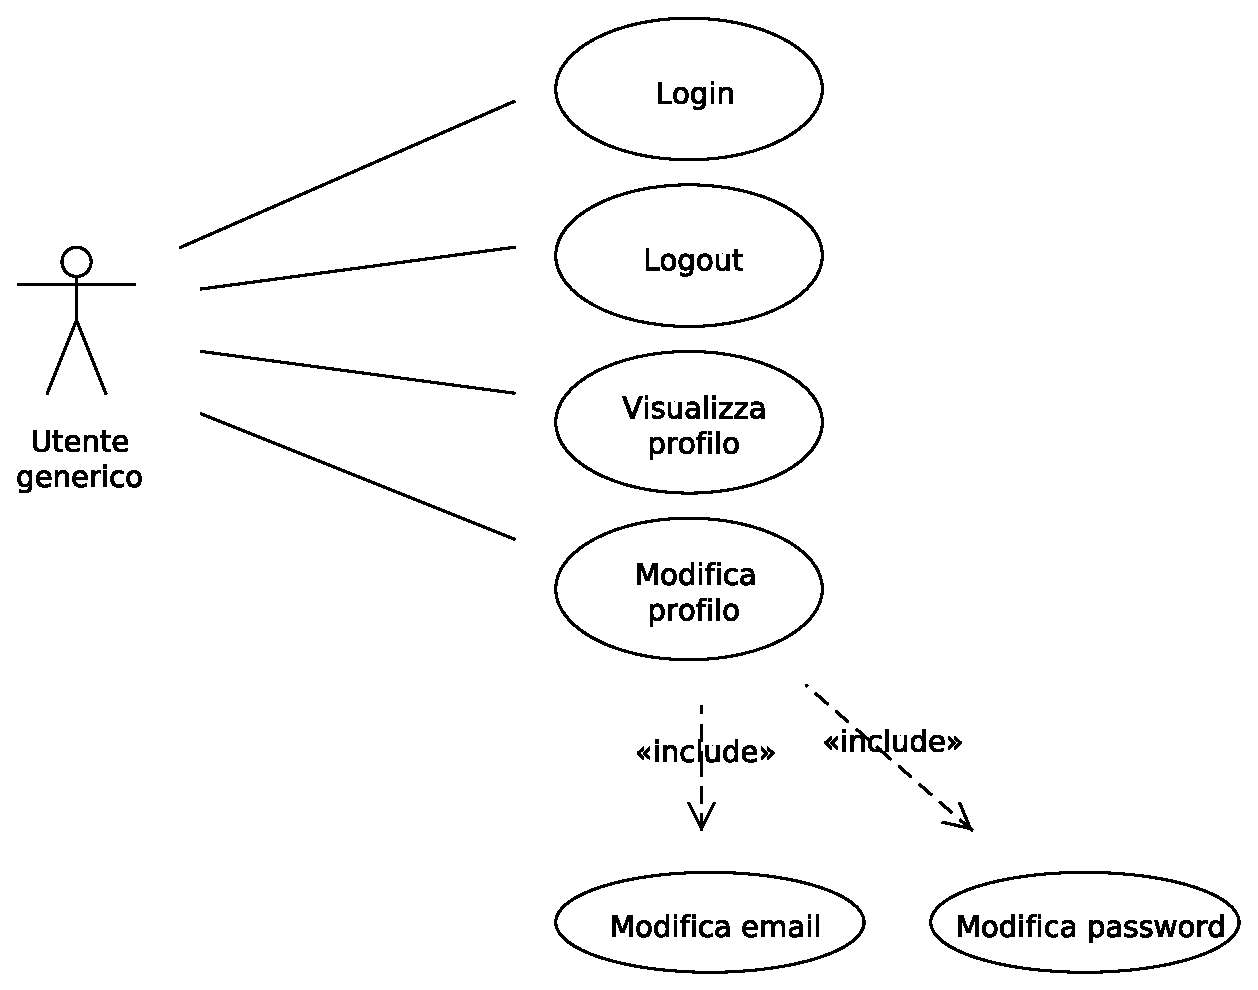
\includegraphics[width=0.7\textwidth]{images/casi_uso_utente_generico.eps}
\end{figure}

\begin{enumerate}

 \item Login\\ \label{UC_login}
    Percorso base:
    l'Utente Generico, dopo aver raggiunto l'indirizzo web dell'applicativo, inserisce il proprio numero di matricola e password, quindi clicca sul pulsante ``Login". Viene visualizzata la pagina iniziale.\\
    Percorso alternativo:
    l' Utente Generico inserisce i propri dati personali ma commette un errore, quindi clicca su ``Login". Viene visualizzato un messaggio nel quale si avvisa l'utente dell'errore commesso.
    
 \item Visualizzazione del profilo\\ \label{UC_view_profile}
    Dopo aver effettuato il login, l'Utente Generico clicca sul pulsante ``Profilo" nella toolbar in alto; si presenta una schermata contente i dati personali dell'Utente.
 \item Modifica dell'indirizzo e-mail\\ \label{UC_edit_email}
  Percorso base:
  dopo aver effettuato il login, l'Utente Generico clicca sul pulsante ``Profilo" nella toolbar in alto; si presenta una schermata contente i dati personali dell'Utente.
  L'Utente cambia il proprio indirizzo e-mail. Una volta effettuate le modifiche desiderate l'Utente clicca su ``Salva". Le modifiche vengono salvate e viene visualizzata la schermata precedente.\\
  
  Percorso alternativo:
  l'Utente inserisce una e-mail non valida. L'Utente è avvertito dell'errore con un messaggio ed è invitato a riprovare.
\end{enumerate}



\item \textbf{Operatore}\\
Una rappresentazione grafica dei casi d'uso dell'Operatore è disponibile in figura \ref{use_case_diag_operator}
\begin{figure}[h]
  \caption{Diagramma dei casi d'uso dell'Operatore}
  \label{use_case_diag_operator}
  \centering
    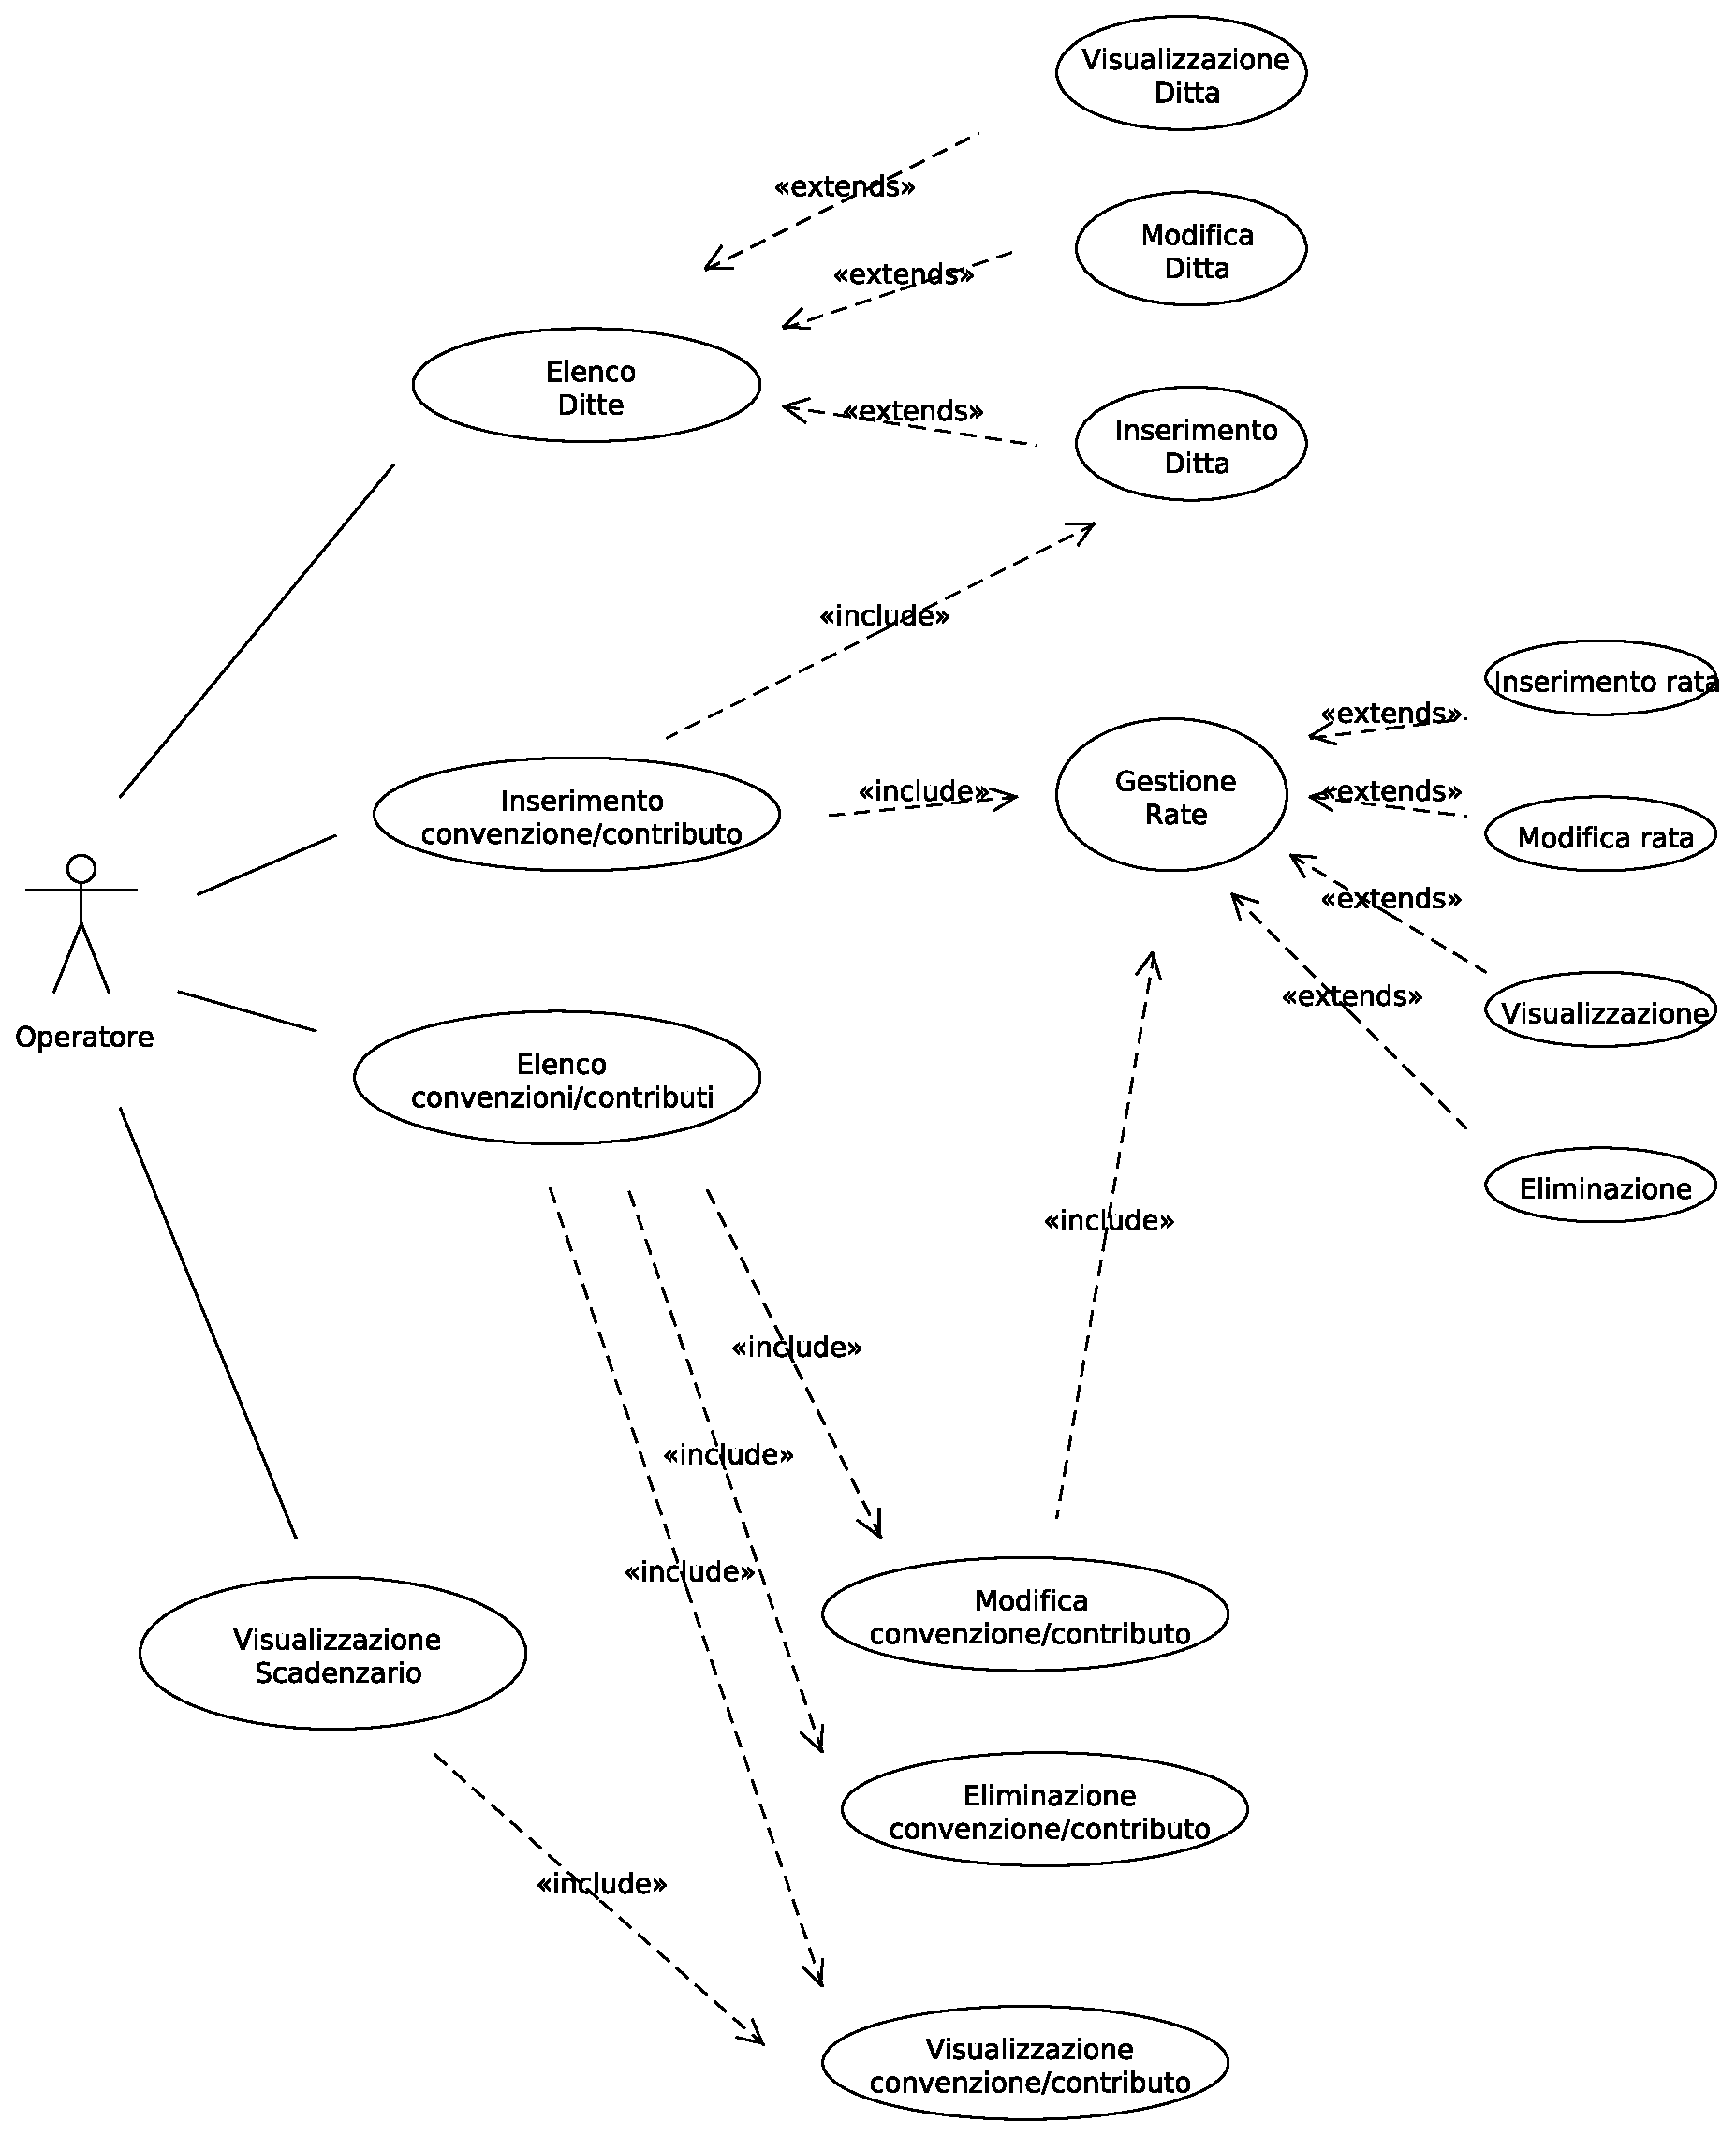
\includegraphics[width=1\textwidth]{images/casi_uso_operatore.eps}
\end{figure}

\begin{enumerate}
  \item Inserimento di una nuova Convenzione/Contributo\\ \label{UC_new_contract}
  
  Percorso base:
  l'Operatore, una volta effettuato il login, clicca su ``Crea una convenzione/contributo"; viene visualizzata una schermata suddivisa in varie schede,
  ognuna corrispondente ad un passo della procedura. E' possibile passare da una vista all'altra mediante i pulsanti ``Avanti" e ``Indietro". I passi sono:
  \begin{enumerate}
    \item Inserimento dei dati della convenzione/contributo\\
      
      In questa scheda sono elencati tutti i campi necessari per la definizione di una convenzione/contributo, 
      che l'Operatore deve compilare. Tali campi sono:
      \begin{itemize}
	\item Il titolo
	\item Il titolo riassuntivo
	\item Il numero di protocollo
	\item L'UAR
	\item La tipologia
	\item Il responsabile scientifico\\
	  Per selezionare un responsabile scientifico è possibile usare l'apposito menù a tendina o, in alternativa, qualora la persona cercata non sia nell'elenco, aggiungerla cliccando sul pulsante ``Aggiungi".
	\item Il referente
	\item La ditta\\
	  Per selezionare una ditta si può usare l'apposito menù a tendina o, se la ditta cercata non fosse presente nell'elenco, aggiungerne una nuova cliccando sul pulsante ``Aggiungi".Per ulteriori dettagli si rimanda \ref{UC_new_company}.
	\item Il nome del progetto CIA
	\item Il Repertorio
	\item Il totale imponibile
	\item L'Iva
	\item La data di approvazione
	\item La data di inizio
	\item La data di scadenza
      \end{itemize}
      
      Nota: i campi riguardanti l'Iva non sono presenti nel caso del contributo.
      
    \item Inserimento della tabella di ripartizione\\
     
      Questa scheda contiene le voci della tabella di ripartizione. L'Operatore può modificare alcuni valori percentuali 
      in base ai quali dividere l'importo totale. Le voci non modificabili sono calcolate in relazione ai campi modificabili facendo riferimento alle norme di Ateneo. Le voci modificabili sono:
      \begin{itemize}
	\item Personale: stabilisce la quota destinata al personale; è l'unico campo principale che l'Operatore può modificare e in base al quale vengono calcolati gli altri.
	\item Missioni, Materiale di consumo, etc. sono sotto-campi di Beni e Servizi e servono per meglio specificare come verrà ripartita la quota destinata a ``Beni e Servizi".
      \end{itemize}
      
      Nota: questa scheda è assente nel caso del contributo, non essendo prevista una ripartizione.
    \item Gestione delle rate\\
      
      Questo passo della procedura è facoltativo: viene data la possibilità all'operatore di inserire delle rate per la convenzione/contributo
      che sta creando. Una volta inserite una o più rate
      queste vengono visualizzate in una tabella e l'Operatore
      ha la possibilità di modificare, visualizzare o eliminare una rata cliccando sui tasti ``Modifica",``Visualizza" ed ``Elimina" che compaiono sulla sinistra, nella riga della tabella
       corrispondente alla rata in questione. Per i dettagli riguardo alle operazioni sulle rate si rimanda ai corrispettivi casi d'uso.

      
    \item Inserimento della documentazione relativa alla convenzione\\
	  
	  Questa scheda elenca i documenti allegati alla convenzione. L'Operatore può aggiungere o eliminare un documento 
	  cliccando sugli appositi tasti. Premendo il tasto ``Salva" la convenzione viene salvata e la procedura termina. Si ritorna alla schermata precedente.
  \end{enumerate}
		 
  Percorso alternativo 1:
  durante uno qualsiasi dei passi, l'Operatore  clicca sul tasto ``Annulla", che comporta, a seguito di una conferma, il ritorno alla schermata precedente
  senza che la convenzione/contributo venga inserita o i cambiamenti effettuati salvati.
  
  Percorso alternativo 2:
  l'Operatore clicca sul tasto ``Salva" senza aver compilato alcuni dei campi obbligatori, o avendo inserito dei valori non consentiti; viene visualizzato un messaggio di errore 
  e il documento non viene salvato. La schermata non viene cambiata, dando la possibilità all'Operatore di procedere alla correzione.
     
  \item Visualizzazione delle convenzioni/contributi\\ \label{UC_view_contract_list}

  Percorso base:
  l'Operatore clicca su ``Visualizza contratti"; viene mostrata una lista delle convenzioni/contributi correntemente stipulate in 
  riferimento al dipartimento di afferenza dell'Operatore, con opportuni filtri 
  per agevolare la ricerca (tra cui un filtro per data di scadenza) e ordinabili per data.
  L'Operatore può selezionare una convenzione e, mediante gli appositi pulsanti che appaiono sulla sinistra, modificare, visualizzare o eliminare una convenzione. Per i dettagli si rimanda casi d'uso relativi a tali operazioni.\\	

  Percorso alternativo:
  l'Operatore clicca sul tasto ``Home", si torna alla pagina iniziale.
 
  \item Modifica di una convenzione/contributo\\ \label{UC_edit_contract}
  
  Percorso base:
  l'Operatore a partire dalla schermata ``Visualizzazione Contratti" clicca sul pulsante ``Modifica" che appare sulla sinistra nella riga 
  della tabella corrispondente alla convenzione/contributo desiderata. Viene visualizzata una schermata suddivisa in schede analoga a quella
  descritta nel caso della ``Creazione di una convenzione/contributo", con la differenza che in questo caso è possibile spostarsi da una scheda all'altra
  cliccando sulla scheda stessa. Inoltre è presente la scheda aggiuntiva ``Riepilogo" che contiene alcune informazioni di riepilogo come il residuo
  totale della convenzione/contributo o il totale fatturato.
  L'Operatore effettua i cambiamenti desiderati quindi clicca sul pulsante ``Salva"; i dati vengono salvati e si ritorna all'elenco delle convenzioni/contributi\\

  Percorso alternativo 1:
  l'Operatore clicca sul tasto \textquotedblleft Annulla" da qualsiasi scheda;  si torna alla schermata \textquotedblleft Visualizzazione Contratti" senza salvare le modifiche effettuate.\\
  
  Percorso alternativo 2:
  l'Operatore clicca su \textquotedblleft Salva" ma alcuni valori immessi non sono corretti, viene visualizzato un messaggio di errore e non si torna alla schermata \textquotedblleft Visualizzazione delle
  convenzioni/contributi" dando la possibilità all'Operatore di correggere gli errori commessi prima di salvare nuovamente.
  
  \item Visualizzazione di una convenzione/contributo\\ \label{UC_view_contract}
 
  Del tutto analogo a ``Modifica di una convenzione/contributo" con la differenza che in questo caso non è possibile modificare i dati della
  convenzione/contributo.
  
  \item Eliminazione di una convenzione/contributo\\ \label{UC_delete_contract}
  
  Percorso base:
  l'Operatore a partire dalla schermata ``Visualizzazione Contratti" clicca sul pulsante ``Elimina" che appare sulla sinistra nella riga 
  della tabella corrispondente alla convenzione/contributo desiderata. Appare una finestra di dialogo che chiede di confermare l'operazione. L'Operatore clicca sul pulsante ``Sì", la convenzione/contributo viene eliminato e si
  ritorna alla schermata precedente.
  
  Percorso alternativo:
  l'Operatore, dopo aver cliccato su ``Elimina", essendosi accorto di aver commesso un errore, clicca sul pulsante ``No". La convenzione/contributo non viene eliminata e si ritorna alla schermata precedente.
  
  
  
\item Inserimento di una rata\\ \label{UC_new_installment}
Percorso base:
l'Operatore può inserire una rata sia in fase di creazione della convenzione/contributo sia in fase di modifica; in entrambi i casi dopo aver raggiunto
la scheda ``Rate" l'Operatore clicca sul pulsante ``Aggiungi una rata".  
Viene visualizzata una finestra di dialogo suddivisa in varie schede,
ognuna corrispondente ad un passo della procedura. E' possibile passare da una scheda all'altra mediante i pulsanti \textquotedblleft Avanti" e \textquotedblleft Indietro". I passi sono:
\begin{enumerate}
  \item Inserimento dei dati della rata\\
  
  L'operatore inserisce i seguenti campi
    \begin{itemize}
    \item Importo
    \item Iva
    \item Data
    \item Numero Reversale
    \item Data Reversale
    \item Numero di Sospeso
    \item Numero di fatturato
    \item Data fatturata
    \item È stata pagata la fattura?
    \item Deve essere allegata la fattura?
    \item Note
    \end{itemize}
    
   Nota: i campi riguardanti l'Iva non sono presenti nel caso del contributo.

   
  \item Inserimento della tabella di ripartizione\\
  
  Il procedimento è del tutto analogo a quello descritto nel caso d'uso \textquotedblleft Inserimento della tabella di ripartizione" per l'inserimento di 
  una nuova convenzione/contributo. 
\end{enumerate}

L'Operatore clicca pulsante \textquotedblleft Salva".Le modifiche vengono salvate e si torna alla schermata precedente;

Percorso alternativo:
l'Operatore clicca sul pulsante ``Annulla", viene chiusa la finestra di dialogo senza che la rata sia stata inserita.

\item Modifica di una rata\\ \label{UC_edit_installment}

Percorso base:
l'Operatore accede alla schermata ``Visualizzazione contratti" cliccando sul pulsante apposito nella pagina iniziale, quindi seleziona la convenzione/contributo alla quale la rata appartiene e clicca sul pulsante ``Modifica" che compare
all'interno della riga selezionata. Viene così visualizzata la schermata ``Modifica di una convenzione/contributo"; l'Operatore raggiunge la scheda ``rate" e clicca sul pulsante ``Modifica" che compare selezionando la riga della tabella
corrispondente alla rata desiderata. Viene visualizzata una finestra di dialogo composta di varie schede analoghe a quelle descritte nel caso dell'inserimento. E' possibile passare da una scheda all'altra cliccando su di esse.
Dopo avere effettuato le modifiche richieste l'Operatore clicca sul pulsante ``Salva", la convenzione/contributo viene aggiornata e viene visualizzata la schermata precedente.

Percorso alternativo:
l'Operatore clicca sul pulsante ``Annulla", le modifiche vengono scartate e si torna alla schermata precedente.

\item Visualizzazione di una rata \label{UC_view_installment}

Una volta raggiunta la scheda ``rate" relativa alla convenzione/contributo di interesse l'Operatore, dopo aver selezionato la rata desiderata, clicca sul pulsante ``Visualizza". Viene presentata una finestra di dialogo analoga a quella descritta nel caso della modifica 
con la differenza che i campi non sono modificabili. E' possibile tornare alla schermata precedente cliccando sul pulsante ``Indietro".

\item Eliminazione di una rata\\ \label{UC_delete_installment}

Raggiunta la scheda ``rate" relativa alla convenzione/contributo di interesse, l'Operatore, dopo aver selezionato la rata di interesse, clicca sul pulsante ``Elimina'; appare una finestra di dialogo che chiede di confermare
l'eliminazione; l'Operatore clicca \textquotedblleft Sì", la rata viene eliminata e si torna alla schermata precedente.

\item Inserimento di una Ditta\\ \label{UC_new_company}
Percorso base:
l'Operatore clicca su ``Visualizza elenco Ditte" dalla pagina iniziale; viene visualizzata una schermata contenente un elenco delle ditte inserite. L'Operatore clicca sul pulsante ``Aggiungi" in basso a sinistra. Viene visualizzata
una finestra di dialogo contente i seguenti campi obbligatori:
\begin{itemize}
 \item Denominazione
 \item Ragione sociale
 \item Sede Legale
 \item Codice fiscale
 \item Partita IVA
\end{itemize}
l'Operatore dopo aver riempito i campi clicca su ``Salva", la nuova ditta viene salvata e si ritorna alla schermata precedente.

Percorso alternativo:
l'Operatore clicca su ``Salva" senza aver riempito tutti i campi obbligatori, viene visualizzato un messaggio di errore che invita l'utente inserire tali campi.

Percorso alternativo 2:
l'Operatore clicca su ``Salva" avendo inserito un codice fiscale di una ditta già inserita. Viene visualizzato un opportuno messaggio di errore.

Percorso alternativo 3:
si può inserire una ditta anche in fase di creazione di una convenzione/contributo cliccando sul pulsante ``Aggiungi" accanto al campo ``ditta" nella scheda ``Dati generali".

\item Modifica di una Ditta\\ \label{UC_edit_company}

Percorso base:
l'Operatore clicca su ``Visualizza elenco Ditte" dalla pagina iniziale; viene visualizzata una schermata contenente un elenco delle ditte inserite. L'Operatore dopo aver posizionato il cursore sulla riga dell'elenco
corrispondente alla ditta di interesse clicca sul pulsante ``Modifica"che appare a sinistra sulla riga selezionata. Viene visualizzata
una finestra di dialogo analoga a quella dell'inserimento.

l'Operatore dopo aver modificato i campi desiderati clicca su ``Salva", la  ditta viene salvata e si ritorna alla schermata precedente.

Percorso alternativo:
l'Operatore clicca su ``Salva" senza aver riempito tutti i campi obbligatori, viene visualizzato un messaggio di errore che invita l'utente a inserire tali campi.

Percorso alternativo 2:
l'Operatore clicca su ``Salva" avendo inserito un codice fiscale di una ditta già inserita. Viene visualizzato un opportuno messaggio di errore.

\item Visualizzazione di una Ditta\\ \label{UC_view_company}
  Percorso base:
  l'Operatore raggiunge l'elenco delle ditte quindi clicca sul pulsante ``Visualizza ditta" che compare sulla sinistra selezionando la riga dell'elenco corrispondente alla ditta desiderata.

\item Visualizzazione dell'elenco delle ditte\\ \label{UC_view_company_list}
  Percorso base:
  l'Operatore dalla pagina iniziale clicca sul pulsante ``Visualizza elenco ditte". Viene presentata una schermata contente un elenco di ditte filtrabili per nome attraverso l'apposito filtro di ricerca.
  
\item Visualizzazione dello Scadenzario\\ \label{UC_view_deadlines}
  Percorso base:
  l'Operatore dalla pagina iniziale clicca sul pulsante ``Visualizza scadenzario". Viene presentata una schermata contente un elenco di contratti che hanno delle rate con scadenze attive. È possibile filtrare i risultati in base a vari
  criteri di ricerca. Selezionando una convenzione/contributo e cliccando sul pulsante ``Visualizza" che compare sulla destra è possibile visualizzare una convenzione/contributo. Per i dettagli su questa operazione si rimanda a \ref{UC_view_contract}

\end{enumerate}

 
\item \textbf{Docente}\\
I casi d'uso del Docente sono rappresentati in figura \ref{use_case_diag_teacher}
\begin{figure}[h]
  \caption{Diagramma dei casi d'uso del Docente}
  \label{use_case_diag_teacher}
  \centering
    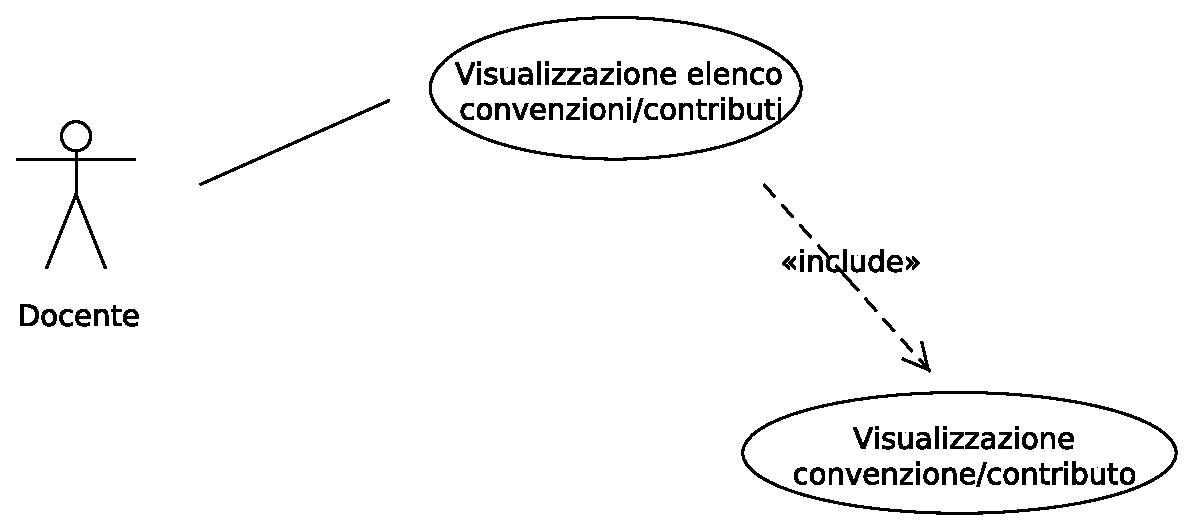
\includegraphics[width=0.8\textwidth]{images/casi_uso_docente.eps}
\end{figure}

\begin{enumerate}
 
 \item Visualizzazione dell'elenco delle convenzioni/contributi di cui il docente è responsabile scientifico\\ \label{UC_view_own_contract_list}
 
 Il docente, dopo aver effettuato il login, può cliccare sul pulsante ``Visualizzazione della lista delle convenzioni/contributi"; la schermata
 che viene visualizzata contiene una tabella che elenca le convenzioni/contributi del docente. E' possibile filtrare le convenzioni/contributi
 secondo vari criteri (data, tipo, scadenze più vicine ...). Inoltre è possibile visualizzare i dettagli di una convenzione/contributo cliccando sul
 pulsante ``Visualizza" che appare posizionando il puntatore su una riga della tabella.
 
 \item Visualizzazione di una convenzione/contributo di cui il docente è responsabile scientifico\\ \label{UC_view_own_contract}
 
 Il docente dalla schermata ``Visualizzazione delle convenzioni/contributi" può cliccare sul pulsante ``Visualizza" relativo ad una convenzione/contributo; compare una schermata suddivisa in schede analoga a quella della modifica/creazione
 della convenzione. Il docente può navigare fra le schede cliccandoci sopra. Non è permessa nessuna modifica ai dati della convenzione/contributo, tuttavia il docente può gestire gli allegati dalla scheda ``Allegati", per i dettagli
 si rimanda a \ref{UC_manage_attachments}. Cliccando su ``Salva"
 gli allegati inseriti dal docente vengono memorizzati, al contrario cliccando su ``Indietro" le modifiche vengono scartate.
 
 \item Gestione allegati\\ \label{UC_manage_attachments}
  
 Percorso base:
 il Docente raggiunge la scheda ``Allegati" di una convenzione/contributo quindi:
  \begin{itemize}
   \item clicca su ``Aggiungi", viene presentata una finestra di dialogo che consente di selezionare un file da inserire come allegato.
   \item clicca sul pulsante ``Download" che compare sulla destra selezionando una riga della tabella degli allegati. Il file corrispondente a tale riga viene scaricato sul computer dell'utente.
   \item clicca sul pulsante ``Rimuovi" che compare sulla destra selezionando una riga della tabella degli allegati. Il file corrispondente viene rimosso dagli allegati della convenzione/contributo
  \end{itemize}
 il docente clicca quindi su ``Salva", le modifiche vengono apportate e si ritorna alla schermata precedente.
 
 Percorso alternativo:
 il Docente, dopo aver effettuato alcune modifiche clicca su ``Indietro", le modifiche non vengono salvate e si ritorna alla schermata precedente.

 
\end{enumerate}



\item \textbf{Amministratore}\\
Una rappresentazione dei casi d'uso dell'Amministratore è disponibile in figura \ref{use_case_diag_admin}
\begin{figure}[h]
  \caption{Diagramma dei casi d'uso dell'Amministratore}
  \label{use_case_diag_admin}
  \centering
    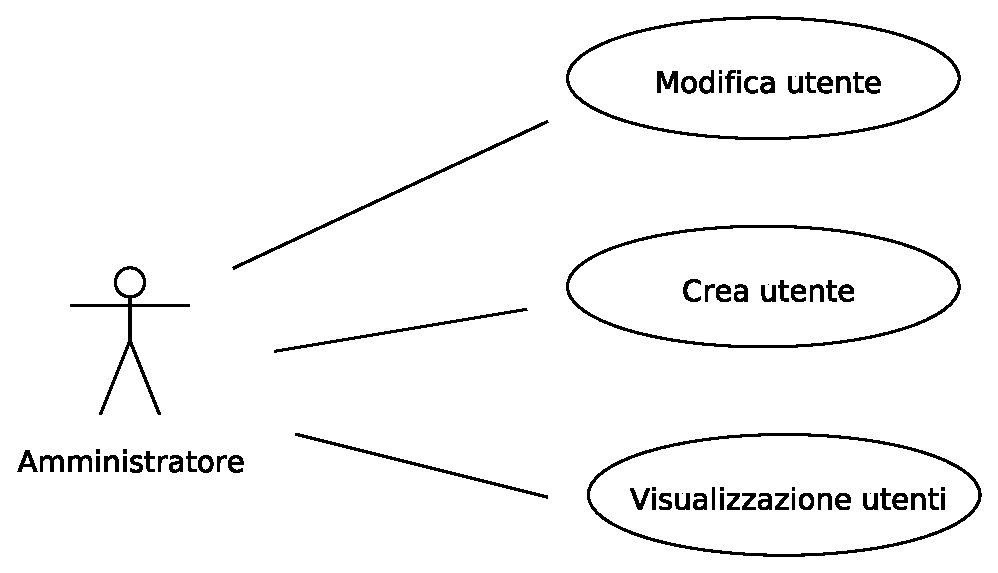
\includegraphics[width=0.6\textwidth]{casi_uso_amministratore.eps}
\end{figure}


\begin{enumerate}
 \item Inserimento di un nuovo utente\\ \label{UC_new_user}
 
 
 Percorso base:
 l'Amministratore, dopo aver effettuato il login, clicca sul pulsante ``Crea nuovo utente"; viene visualizzata una schermata che permette
 di inserire i dati dell'utente:
 \begin{itemize}
  \item Nome
  \item Cognome
  \item Matricola
  \item E-mail
  \item	Password\\
    In realtà i campi che l'Amministratore deve riempire sono due: un campo password ed un campo di verifica che deve corrispondere col precedente.
  \item Ruolo\\
    L'Amministratore può scegliere il ruolo dal rispettivo menù a tendina, i ruoli disponibili sono Operatore, Amministratore, Docente.
 \end{itemize}
 
 Una volta completato l'inserimento, l'Amministratore clicca sul pulsante ``Salva", il nuovo utente viene registrato nel sistema. 

 Percorso alternativo 1:
 l'Amministratore inserisce solo il campo matricola e quindi clicca il pulsante ``Importa Utente da LDAP". I rimanenti campi, se la matricola è valida,
 vengono automaticamente importati dal servizio LDAP offerto da SIAF. L'Amministratore conclude la procedura cliccando sul pulsante ``Salva"
 
 Percorso alternativo 2:
 l'Amministratore in qualunque momento della procedura clicca sul pulsante ``Annulla"; viene presentata a video la schermata precedente,
 nessun utente viene aggiunto al sistema.
 
 \item Visualizzazione della lista degli utenti \label{UC_view_user_list}
  L'Amministratore, una volta effettuato il login, clicca sul pulsante ``Visualizza utenti"; viene presentata una schermata contenente una lista  degli
  utenti inseriti nel sistema. L'Amministratore clicca sul pulsante ``Indietro" per tornare alla pagina iniziale.
\end{enumerate}

\item \textbf{Tempo}\\
I casi d'uso del Tempo sono rappresentati in figura \ref{use_case_diag_teacher}
\begin{figure}[h]
  \caption{Diagramma dei casi d'uso del Tempo}
  \label{use_case_diag_time}
  \centering
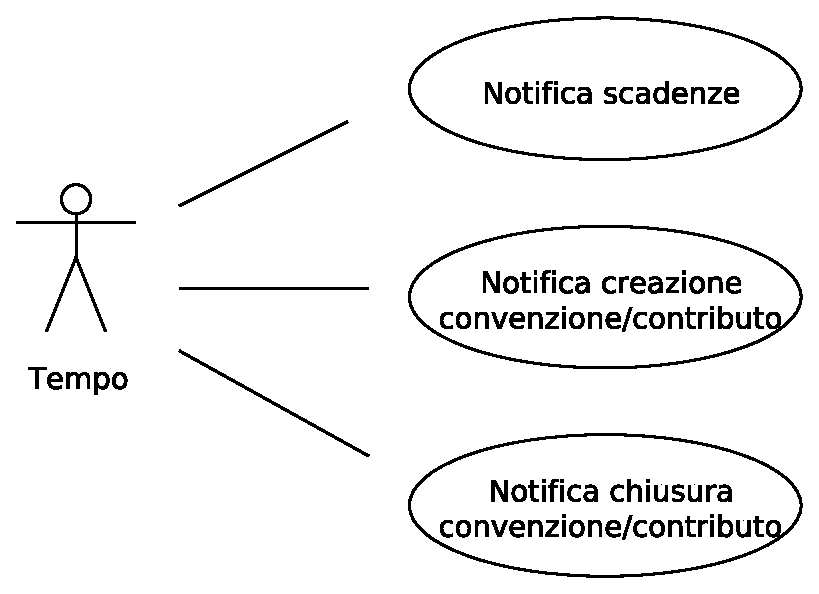
\includegraphics[width = 0.5\textwidth]{images/casi_uso_tempo.eps}
\end{figure}
\begin{enumerate}
 \item Notifica delle scadenze\\ \label{UC_notify_deadlines}
 
    Ad intervalli periodici stabiliti, i docenti che hanno convenzioni/contributi attive con rate in scadenza ravvicinata, vengono avvertiti tramite posta elettronica.
  
 
 \item Notifica della creazione di una nuova convenzione/contributo\\ \label{UC_notify_new_contract}
 
    Al momento del completamento della creazione di una nuova convenzione/contributo viene inviata una e-mail all'indirizzo di posta elettronica del responsabile scientifico indicato per la convenzione/contributo. Tale e-mail contiene
    le informazioni principali che caratterizzano la convenzione/contributo.
  
  
 \item Notifica della chiusura di una convenzione/contributo\\ \label{UC_notify_closed_contract}
 
    Al momento della chiusura di una convenzione/contributo (ovvero quando il fatturato è pari all'importo totale) viene inviata, all'indirizzo di posta elettronica del responsabile scientifico, una e-mail che notifica la chiusura della convenzione/contributo, riportando alcuni dati della stessa.
\end{enumerate}


\end{enumerate}

